\pagebreak

\textsc{\begin{figure}[htbp!]
    \centering
        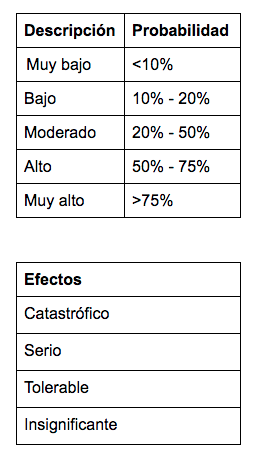
\includegraphics[width=0.3\textwidth]{images/riesgos}
    \caption{Especificaciones de riesgos}
\end{figure}}
\section{Tabla de Riesgos}
\begin{riesgos}
\riesgo{El cliente cambia los requerimientos }{Alto
}{Catastrófico}
\riesgo{La base de datos no es compatible con la información que usan actualmente}{Alto}{Catastrófico}
\riesgo{Baja capacidad de los equipos de cómputo de los analistas}{Moderado}{Catastrófico}
\riesgo{Falta de información acerca de las capacidades del servidor}{Bajo}{Catastrófico}
\riesgo{Mala proyección del alcance del proyecto}{Bajo}{Catastrófico}
\riesgo{Incompatibilidad con distintos navegadores}{Alto}{Serio}
\riesgo{Incompatilivdad con la versión del navegador}{Alto}{Serio}
\riesgo{Falla en la conexión a internet}{Moderado}{Serio}
\riesgo{Información ambigua del cómo laboran actualmente los analistas}{Moderado}{Serio}
\riesgo{El tiempo para desarrollar el software es insuficiente}{Bajo}{Serio}
\riesgo{El personal clave no está disponible en momentos críticos por razones externas}{Bajo}{Serio}
\riesgo{Las reuniones del equipo no son suficientes }{Bajo}{Serio}
\riesgo{Falta de organización del equipo de trabajo}{Bajo}{Serio}
\riesgo{Actualización de la interfaz gráfica de la página web de ESCOM}{Muy Alto}{Tolerable}
\riesgo{Ocupaciones ajenas al proyecto por parte de los integrantes del Scrum team}{Alto}{Tolerable}
\riesgo{Falta de experiencia en tecnologías solicitadas}{Moderado}{Tolerable}
\riesgo{Mayor número de usuarios de lo planificado}{Bajo}{Tolerable}
\riesgo{Cambio de personal encargado de los trámites}{Bajo}{Tolerable}
\riesgo{Baja moral del personal, malas relaciones entre miembros del equipo}{Baja}{Tolerable}
\riesgo{La organización se reestructura y una nueva administración se responsabiliza del proyecto.}{Baja}{Tolerable}

\end{riesgos}